\FloatBarrier
\subsection{Question 4}
In this section, we mirror one of the zeros to a location outside the unit circle, as shown in \autoref{code:pp41}. The poles and zeros of the modified system are illustrated in \autoref{fig:pp41}. The step response of the system with the mirrored zero is presented in \autoref{fig:pp42}, while the system’s response to the pulse input is shown in \autoref{fig:pp43}.

\begin{code}
	\begin{matlabcode}{firstnumber = 9}
	G_mirrored = ((5*((0.7*s)+1)*(s-0.8))/((((3*s)+1)^2)*((2*s)-1)));
	Gz = c2d(G_mirrored, sampleTimeIntervals, 'zoh');
	\end{matlabcode}
	\captionof{listing}{Poles \& zeros with a mirrored zero}
	\label{code:pp41}
\end{code}

\begin{figure}
	\centering
	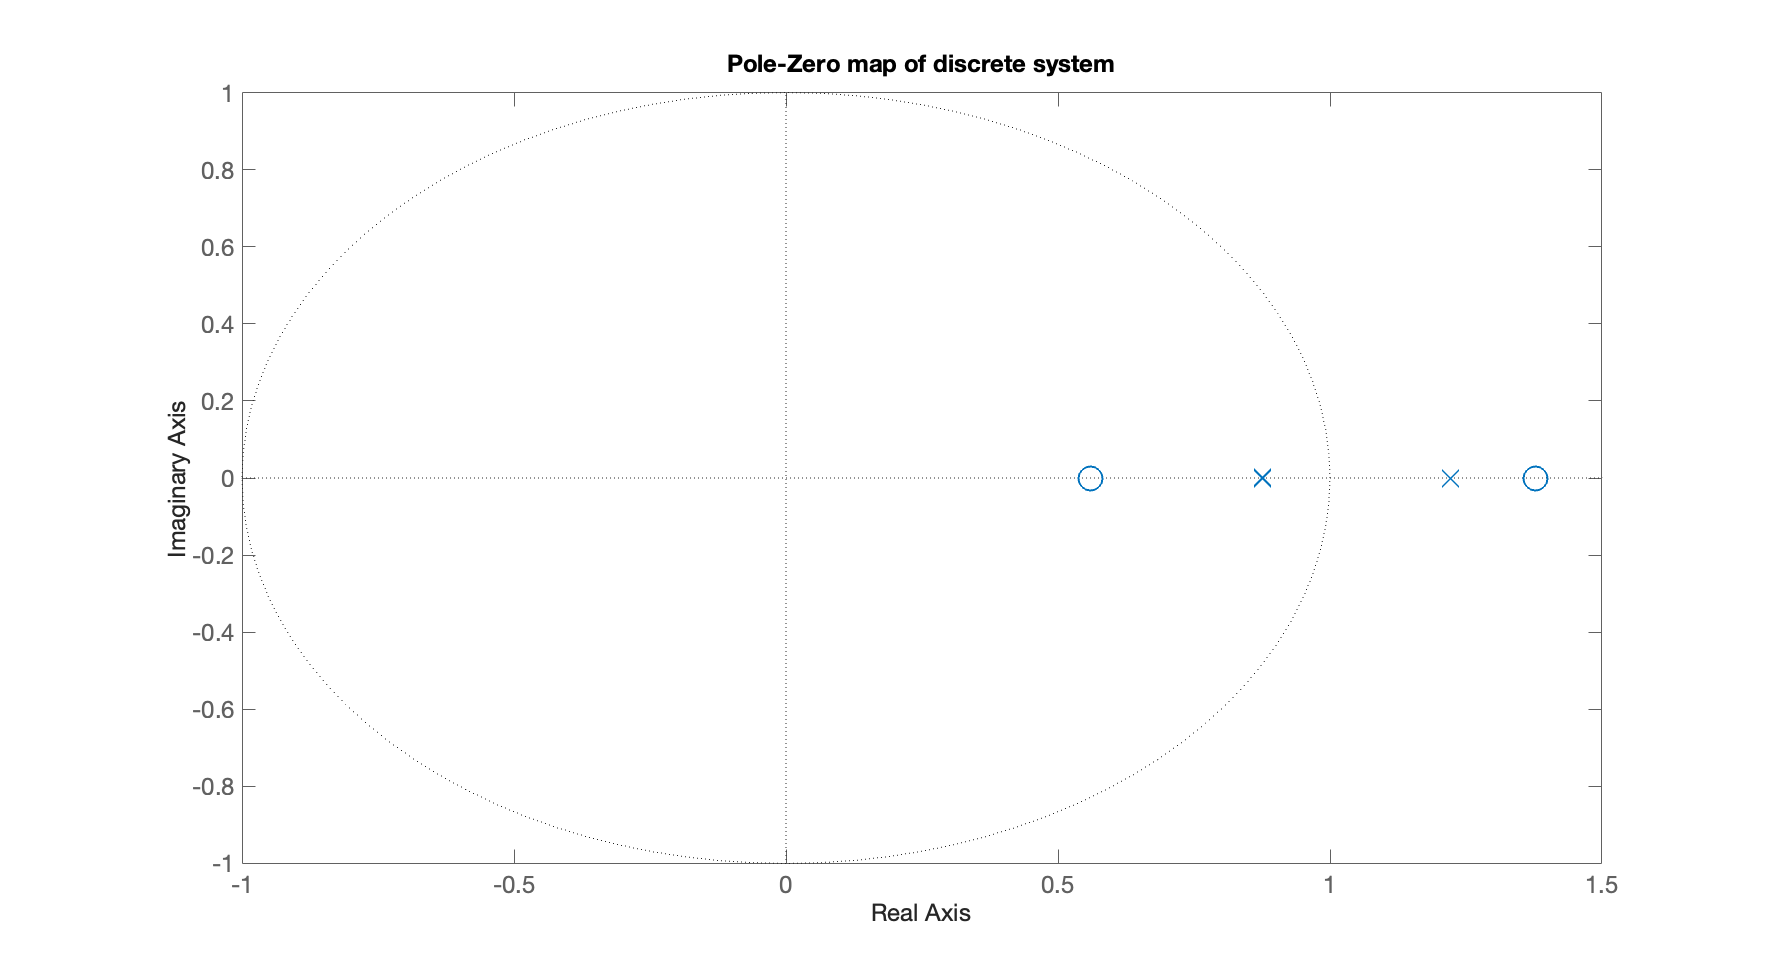
\includegraphics[width=\textwidth]{images/pp41.png}
	\caption{Step response of system with mirrored zero}
	\label{fig:pp41}
\end{figure}

\begin{figure}
	\centering
	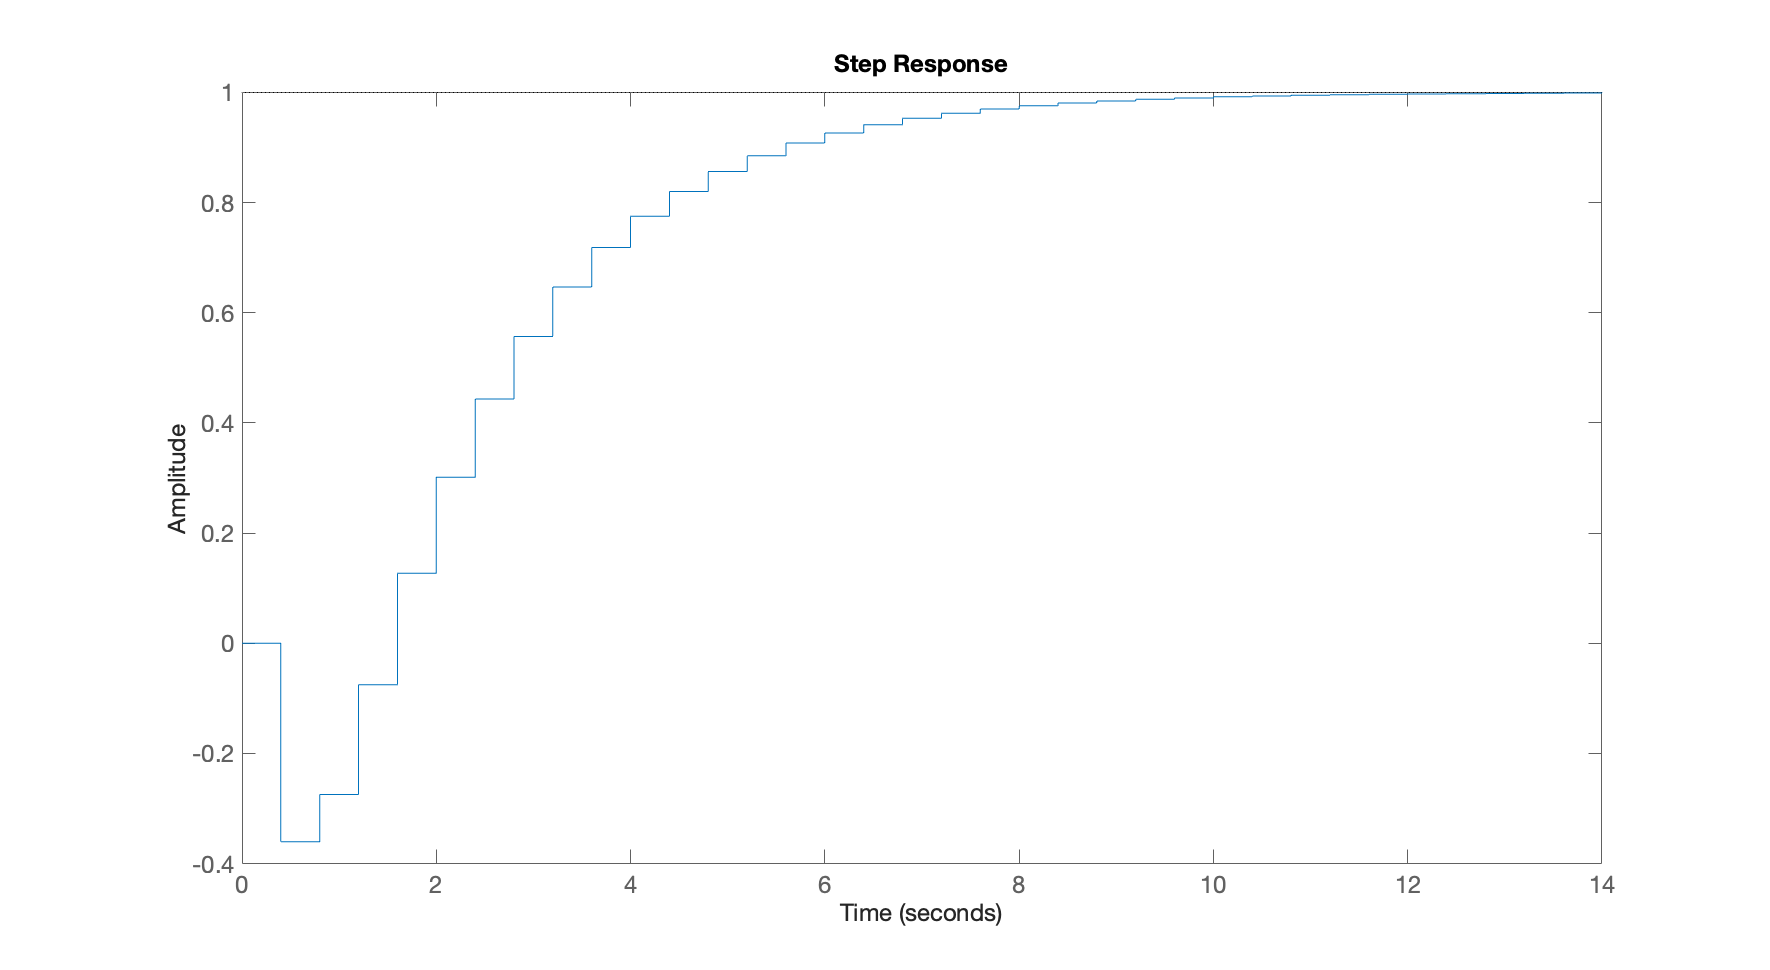
\includegraphics[width=\textwidth]{images/pp42.png}
	\caption{Pulse response of closed system without cancellation}
	\label{fig:pp42}
\end{figure}

\begin{figure}
	\centering
	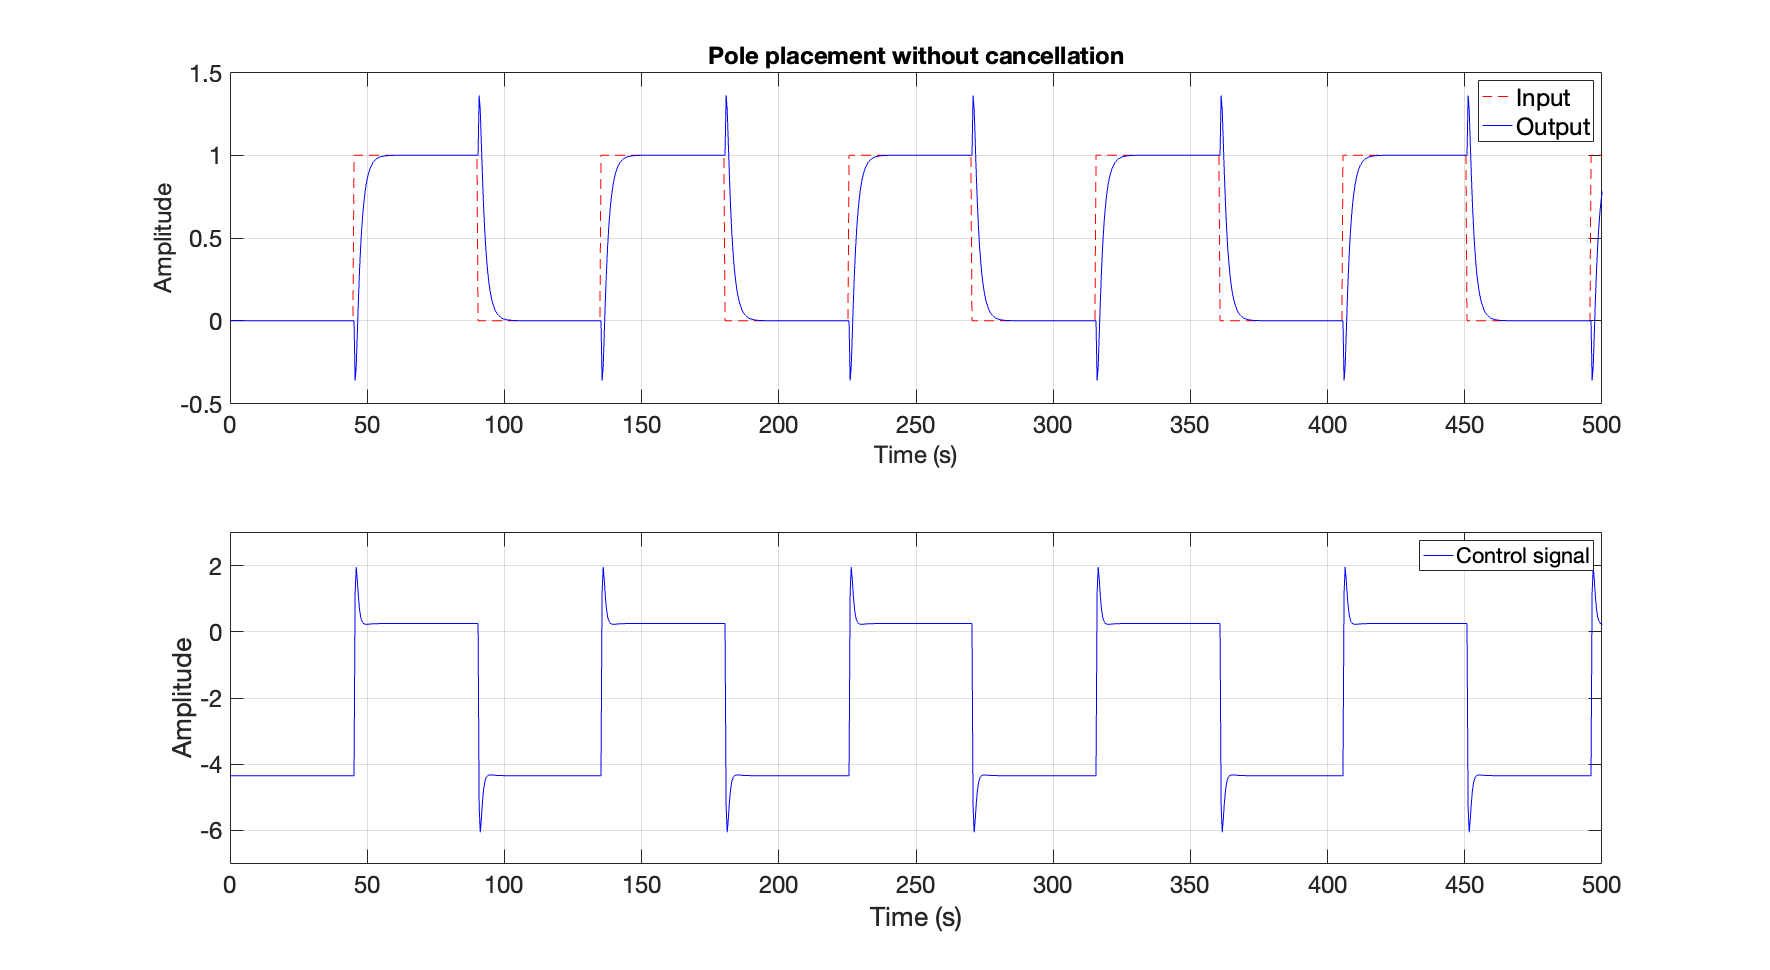
\includegraphics[width=\textwidth]{images/pp43.png}
	\caption{Pulse response of system with mirrored zero}
	\label{fig:pp43}
\end{figure}

\noindent The code  for this section is available at \lstinline|assignment2/part1/PP1_4.m|. 

